\subsection {Session 10, Exercise 1}

\lineparagraph {Exercise}

Let the weights in problem $BINPACKING$ be $s_1 = 0.4; s_2 = 0.7; s_3 = 0.1; s_4 = 0.5$. Perform in this case

\begin{enumerate}[a)]
    \item algorithm $FF$
    \item algorithm $FFD$
\end{enumerate}

\begin{itemize}
    \item How many bins are used by an optimal packing?
    \item What if the last weight changed to $s_4' = 0.6$?
\end{itemize}

\lineparagraph {Solution}

\begin{itemize}
    \item In all binpacking exercises the bins are of size $1.0$, while weights can be between $0<s_i\leq{}1$.
\end{itemize}

\textbf{FF}

\begin{itemize}
    \item $FF$, or first fit will iterate over the given weights, in the order which they are given and will try to fit it to the first available bin. If there is no bin, into which it would fit, then it opens a new bin.
    \item For the first weight of $0.4$, $FF$ opens a new bin.
\end{itemize}

\begin{center}
    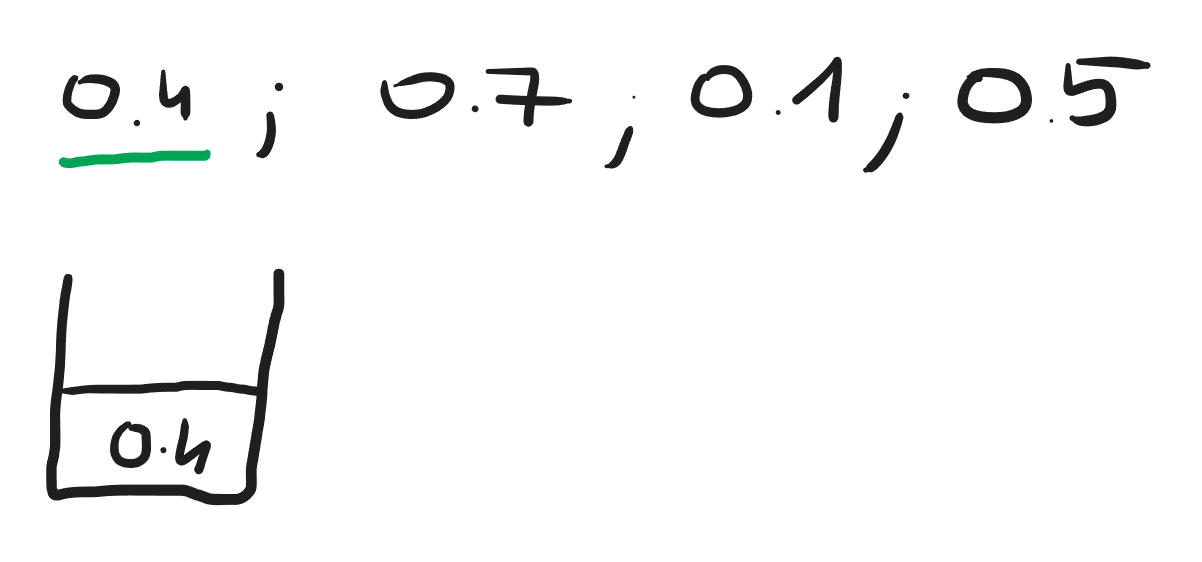
\includegraphics[width=0.5\linewidth]{10/01/ff_01.png}
\end{center}

\begin{itemize}
    \item For $0.7$ we must open a new bin, since $0.4+0.7=1.1$, so they won't fit into a single bin.
\end{itemize}

\begin{center}
    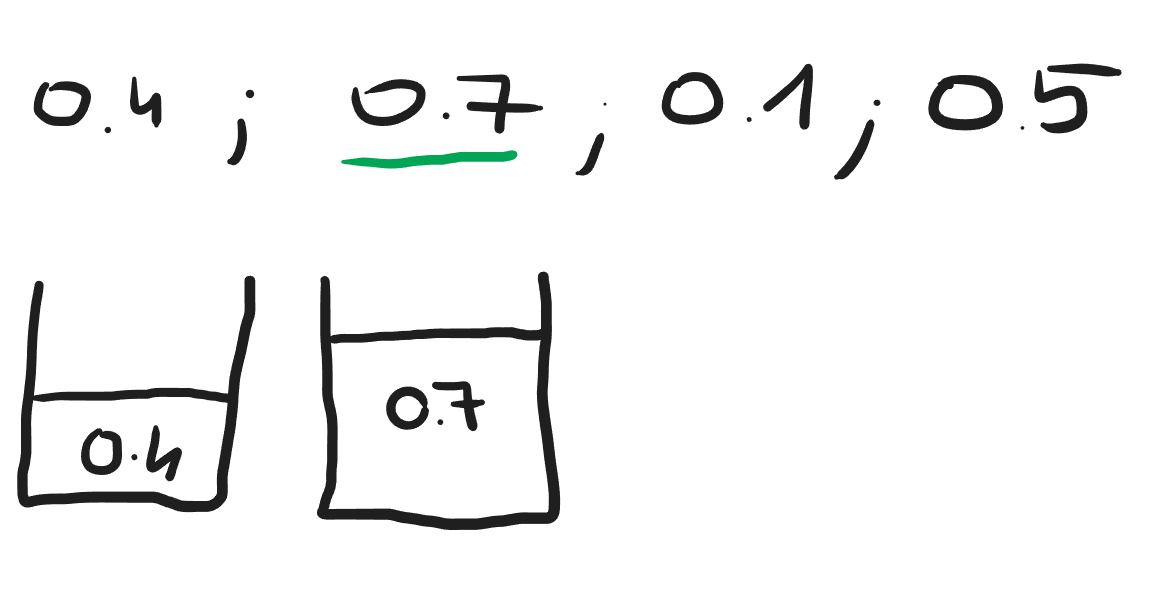
\includegraphics[width=0.5\linewidth]{10/01/ff_02.png}
\end{center}

\begin{itemize}
    \item $0.1$ fits immediately into the first bin, next to the $0.4$, so the algorithm will put it there and will not try further bins.
\end{itemize}

\begin{center}
    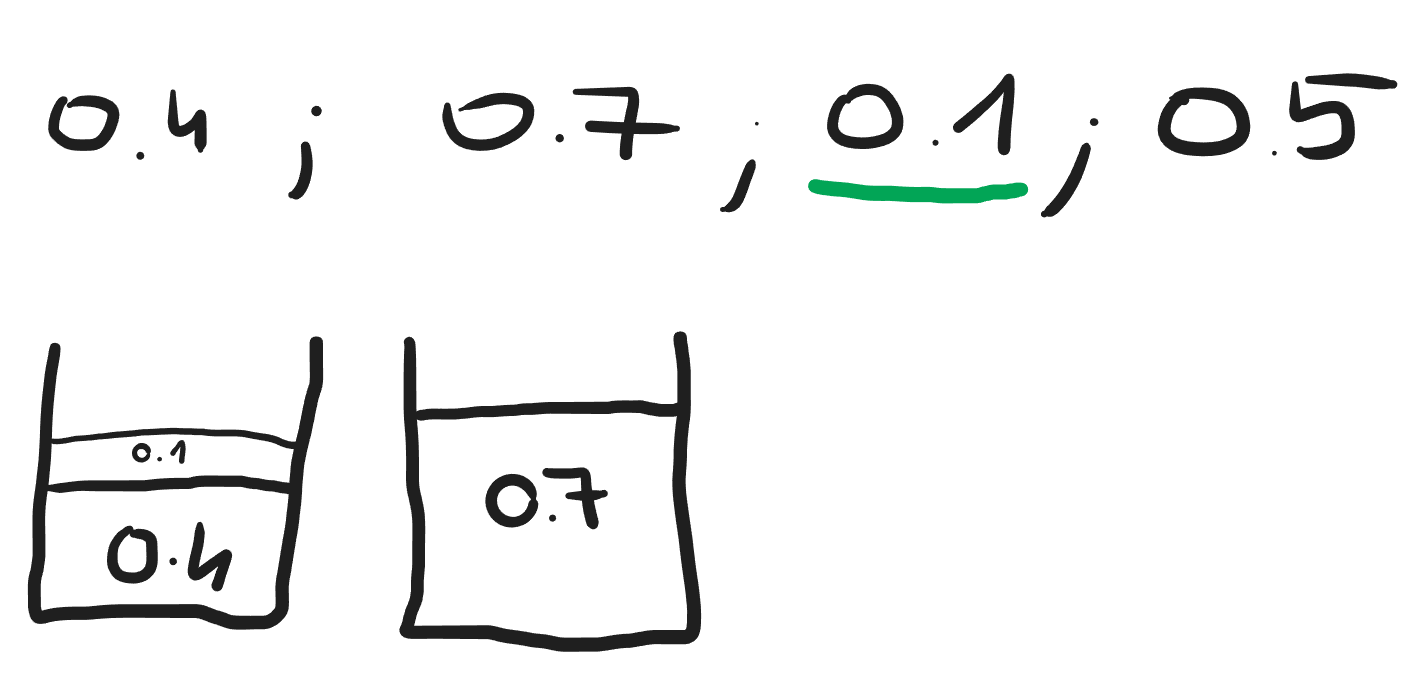
\includegraphics[width=0.5\linewidth]{10/01/ff_03.png}
\end{center}

\begin{itemize}
    \item $0.5$ fits next to $0.1+0.4$, since $0.1+0.4+0.5=1.0$, so they fill the first bin exactly!
\end{itemize}

\begin{center}
    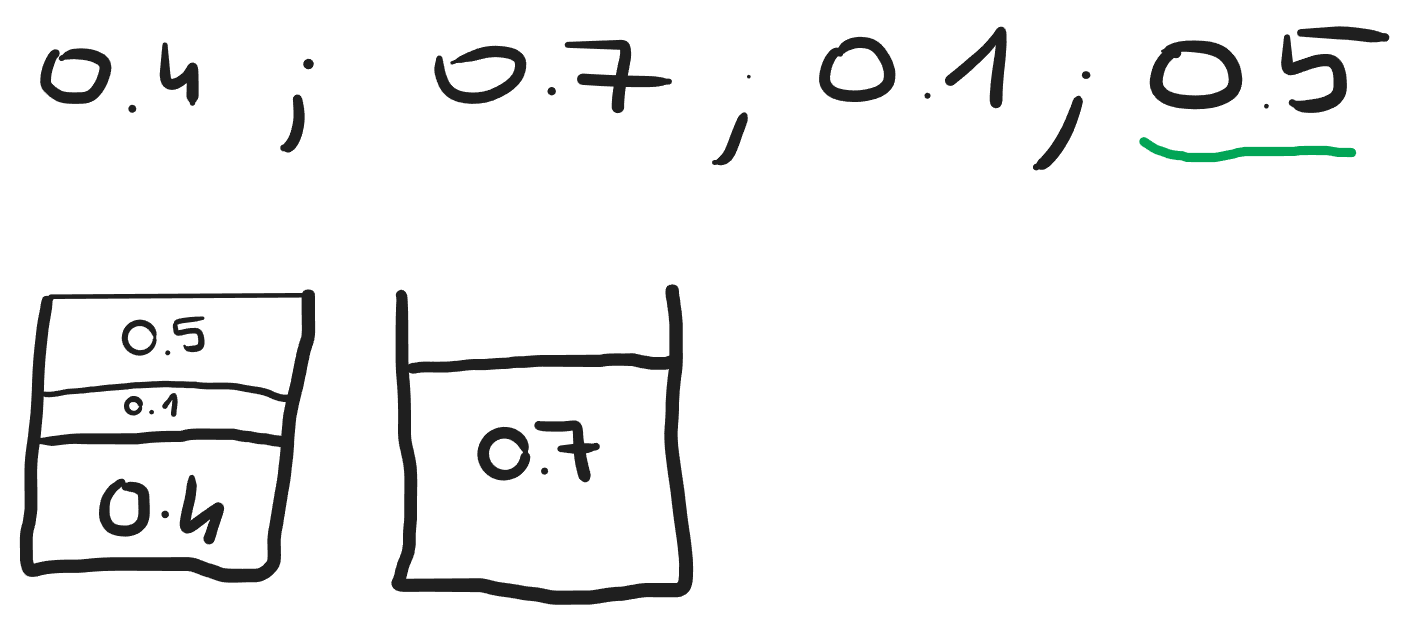
\includegraphics[width=0.5\linewidth]{10/01/ff_04.png}
\end{center}

\textbf{FF with $s_4'=0.6$}

\begin{itemize}
    \item The first three weights are placed the same way as previously, since nothing changed here.
\end{itemize}

\begin{center}
    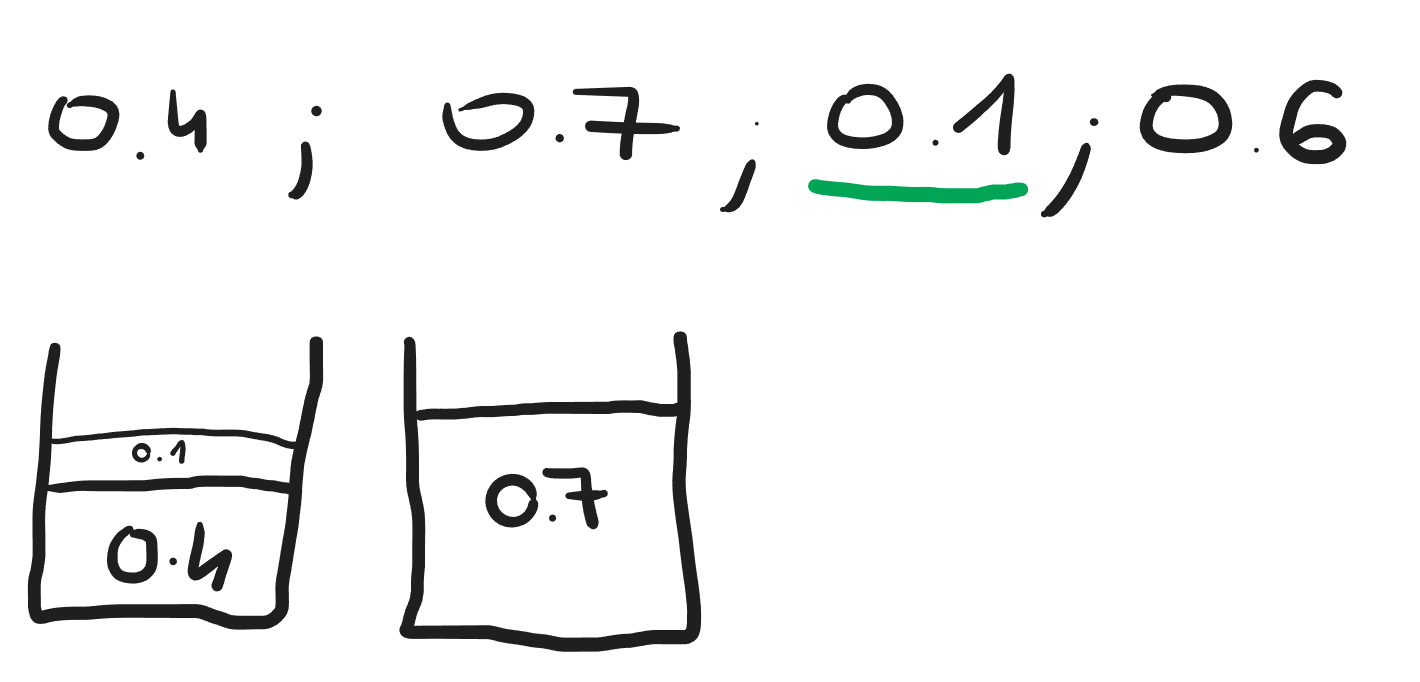
\includegraphics[width=0.5\linewidth]{10/01/ff_alt_03.png}
\end{center}

\begin{itemize}
    \item $0.6$ will not fit next to $0.1+0.4$, since $0.1+0.4+0.6=1.1$, neither next to $0.7$, since $0.7+0.6=1.3$ so we need to open a new bin for it!
\end{itemize}

\begin{center}
    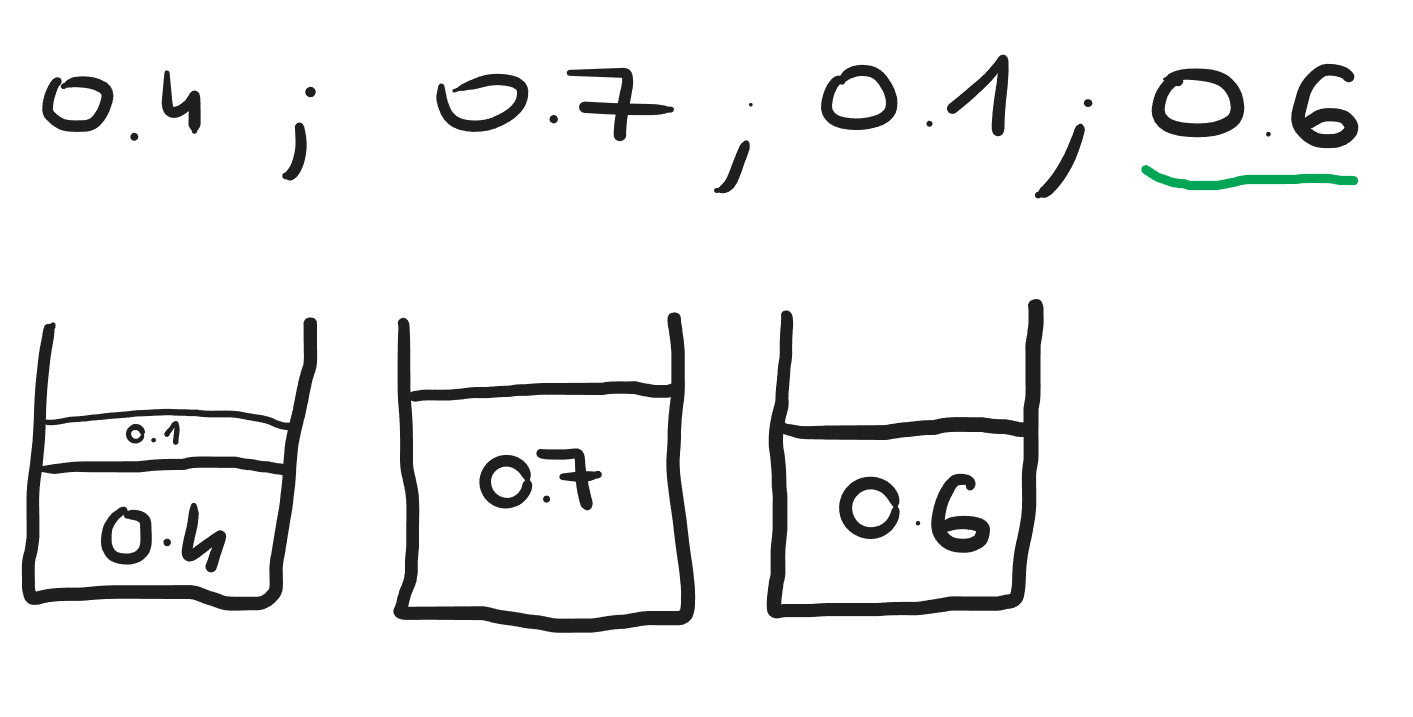
\includegraphics[width=0.5\linewidth]{10/01/ff_alt_04.png}
\end{center}

\textbf{FFD}

\begin{itemize}
    \item $FFD$, or first fit decreasing will first sort the weights in decreasing order, then iterate over them in this order and will try to fit the current item to the first available bin. If there is no bin, into which it would fit, then it opens a new bin.
    \item For the first weight of $0.7$, $FFD$ opens a new bin.
\end{itemize}

\begin{center}
    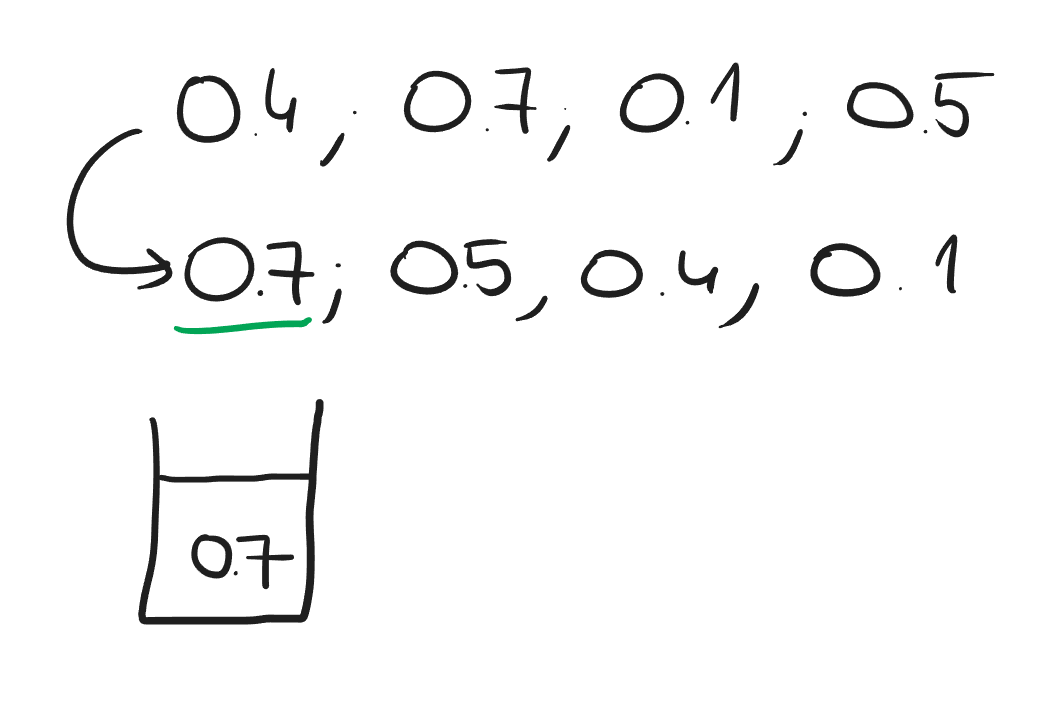
\includegraphics[width=0.5\linewidth]{10/01/ffd_01.png}
\end{center}

\begin{itemize}
    \item For $0.5$ we must open a new bin, since $0.5+0.7=1.2$, so they won't fit into a single bin.
\end{itemize}

\begin{center}
    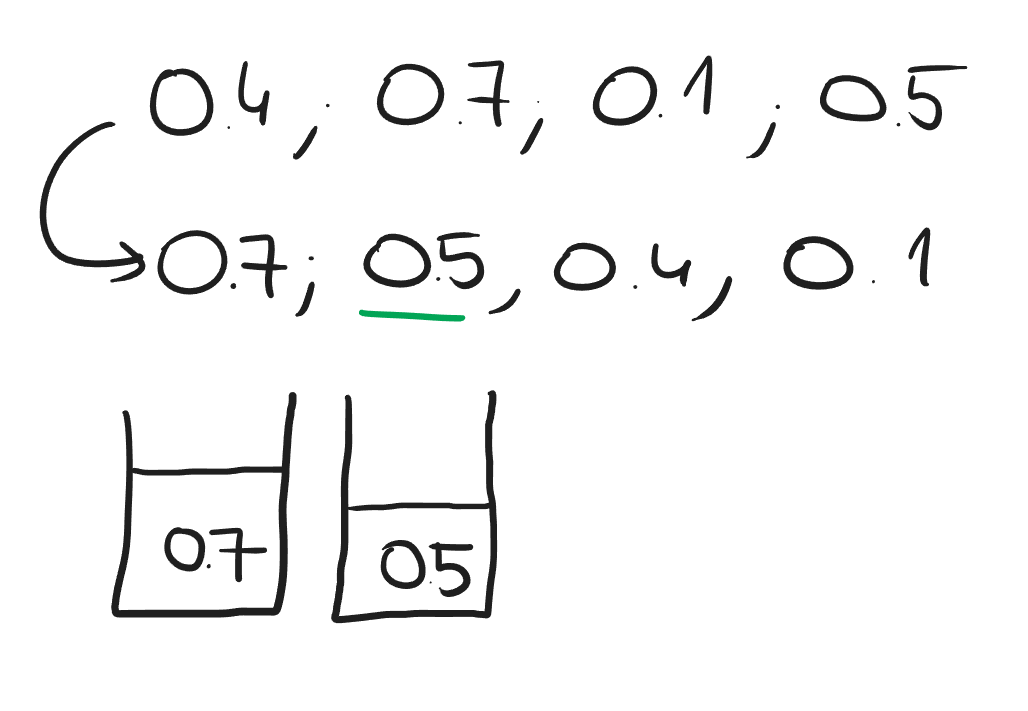
\includegraphics[width=0.5\linewidth]{10/01/ffd_02.png}
\end{center}

\begin{itemize}
    \item $0.4$ won't fit next to $0.7$, since $0.7+0.4=1.1$, however it fits next to $0.5$, since $0.5+0.4=0.9$, so we put it there.
\end{itemize}

\begin{center}
    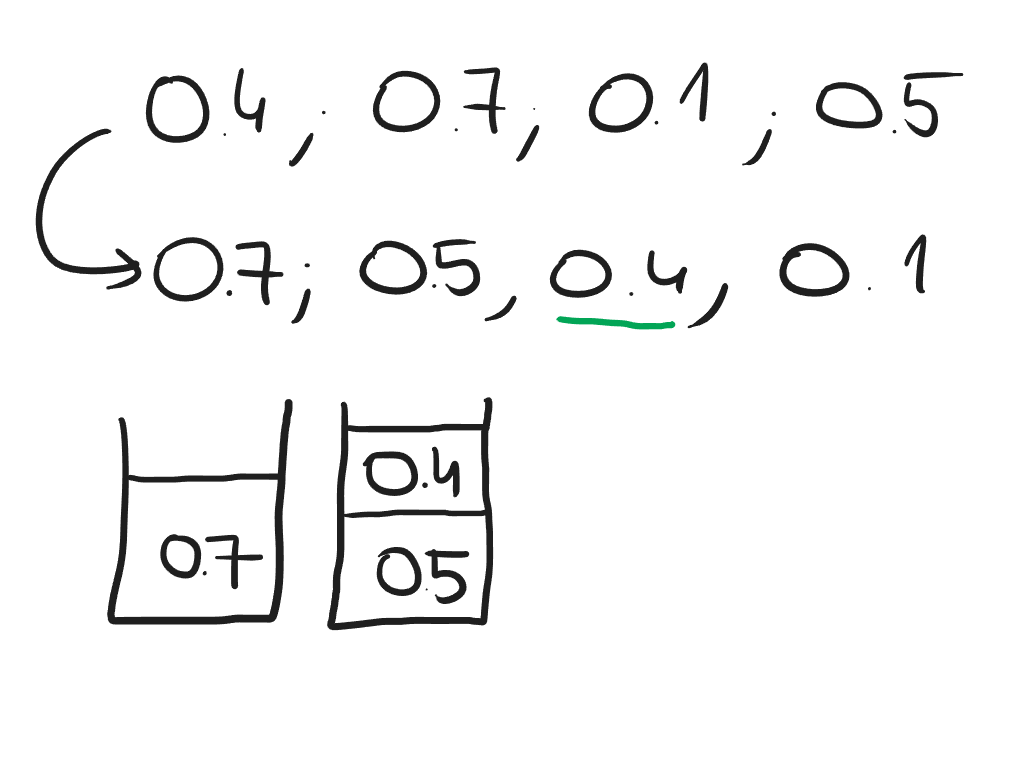
\includegraphics[width=0.5\linewidth]{10/01/ffd_03.png}
\end{center}

\begin{itemize}
    \item Finally, $0.1$ fits immediately next to $0.7$, since $0.7+0.1=0.8$, so the algorithm stops here!
\end{itemize}

\begin{center}
    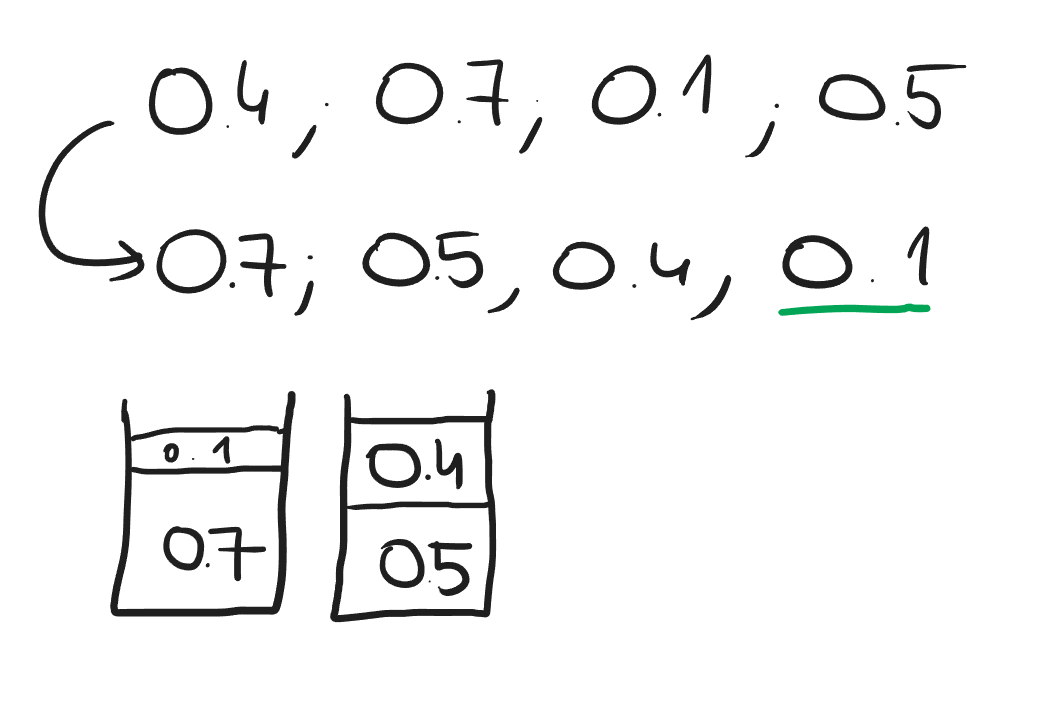
\includegraphics[width=0.5\linewidth]{10/01/ffd_04.png}
\end{center}

\textbf{FFD with $s_4'=0.6$}


\begin{itemize}
    \item $FFD$ sorts the weights again and opens a new bin for the first weight of $0.7$.
\end{itemize}

\begin{center}
    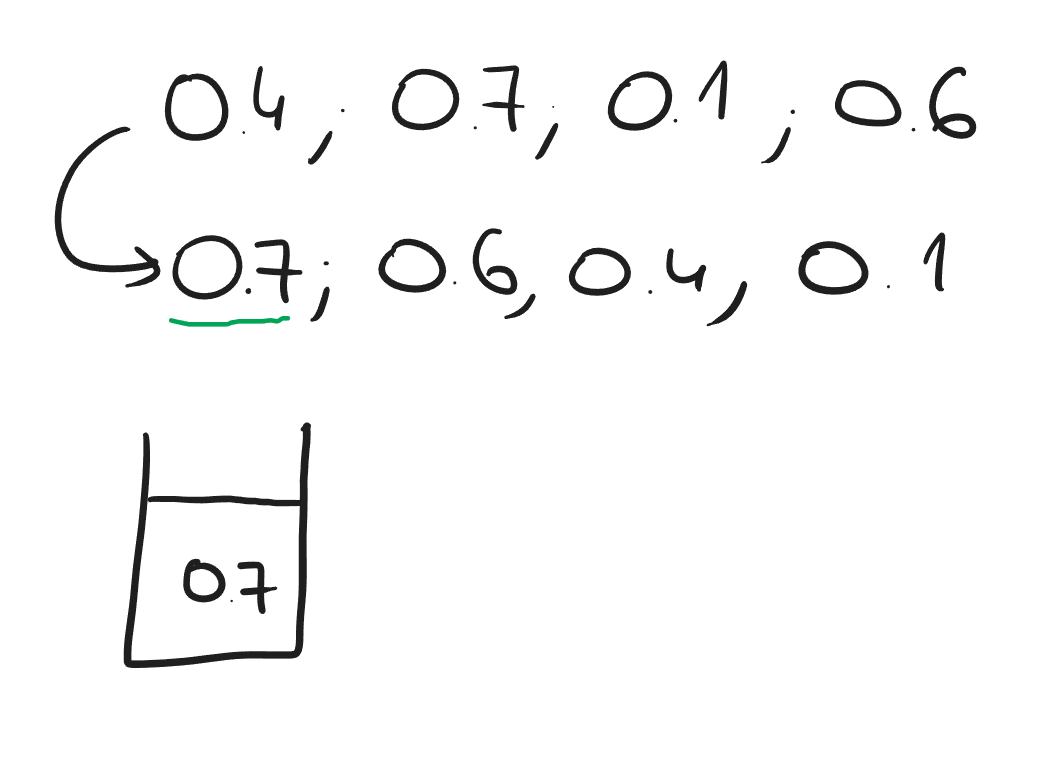
\includegraphics[width=0.5\linewidth]{10/01/ffd_alt_01.png}
\end{center}

\begin{itemize}
    \item For $0.6$ we must open a new bin, since $0.6+0.7=1.3$, so they won't fit into a single bin.
\end{itemize}

\begin{center}
    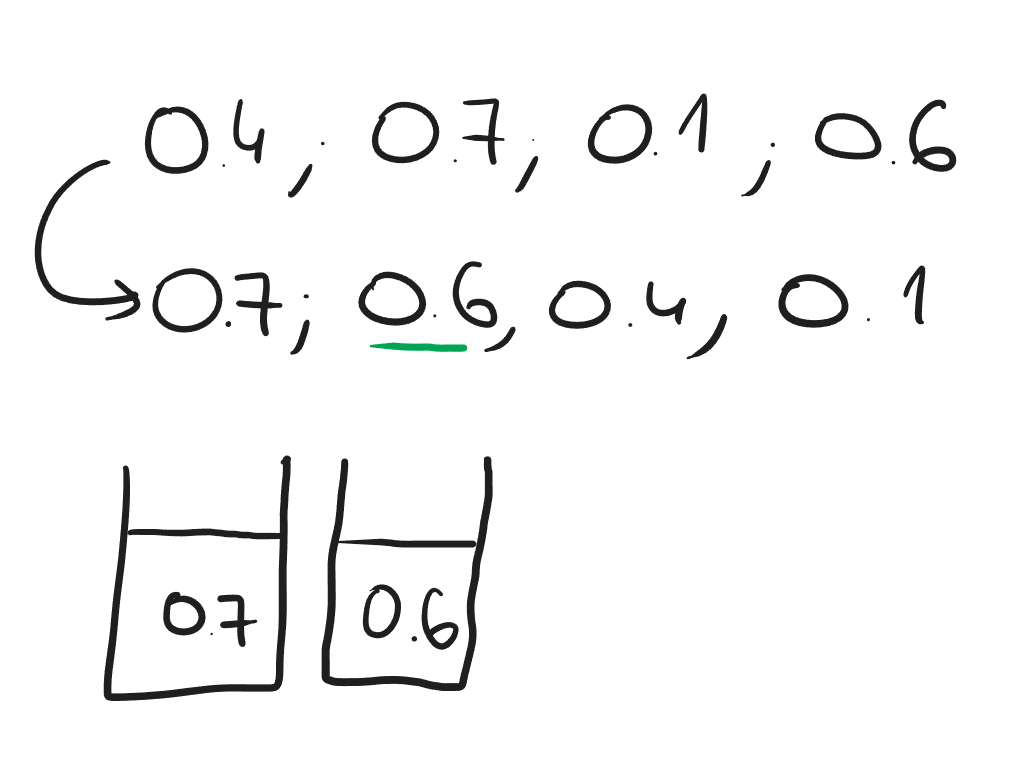
\includegraphics[width=0.5\linewidth]{10/01/ffd_alt_02.png}
\end{center}

\begin{itemize}
    \item $0.4$ won't fit next to $0.7$, since $0.7+0.4=1.1$, however it fits next to $0.6$, since $0.6+0.4=1.0$, so we put it there.
\end{itemize}

\begin{center}
    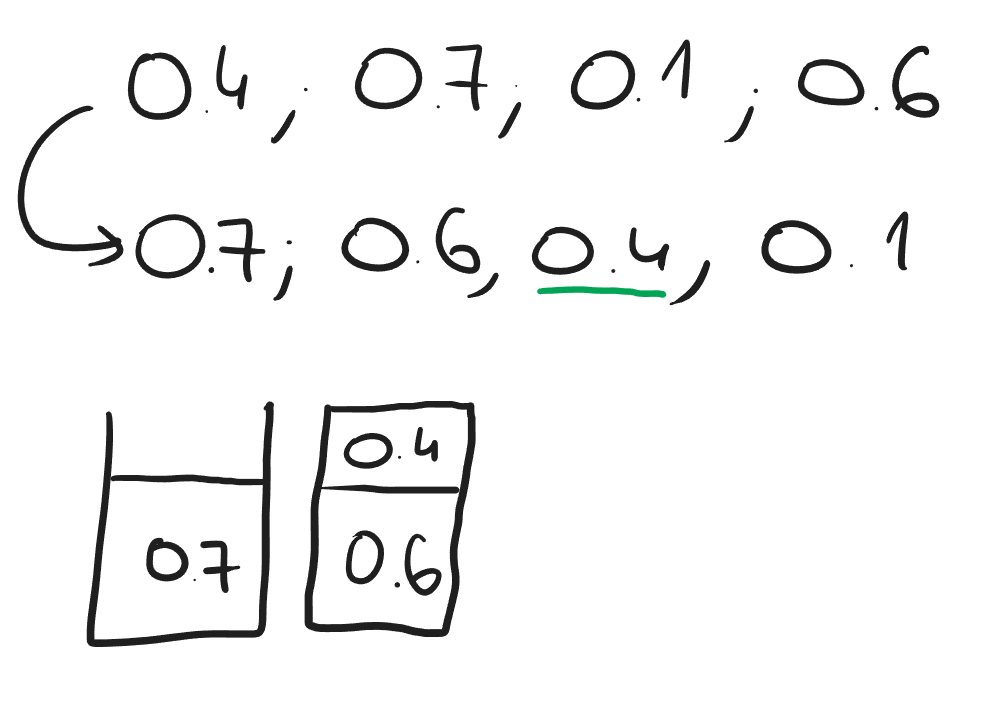
\includegraphics[width=0.5\linewidth]{10/01/ffd_alt_03.png}
\end{center}

\begin{itemize}
    \item Finally, $0.1$ fits next to $0.7$, since $0.7+0.1=0.8$, so we put it into the first bin and the algorithm stops here!
\end{itemize}

\begin{center}
    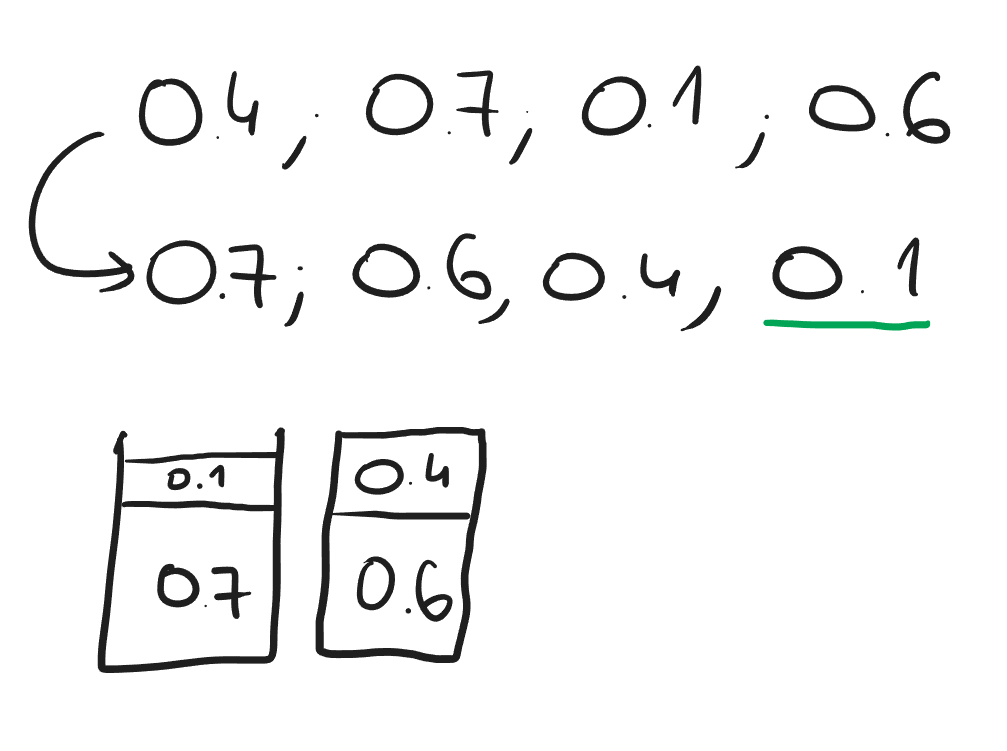
\includegraphics[width=0.5\linewidth]{10/01/ffd_alt_04.png}
\end{center}

\textbf{The optimal solutions}

\begin{itemize}
    \item For weights $0.4$, $0.7$, $0.1$ and $0.5$, the optimal solution uses $2$ bins, for example the first bin $0.1+0.4+0.5=1.0$ and the second bin $0.7$. We know this is an optimal solution, because every single bin, except (maybe) the last one is filled fully, so there is no possible way to compress this further! Both $FF$ and $FFD$ finds an optimal solution, which uses two bins.
    \item For weights $0.4$, $0.7$, $0.1$ and $0.6$, the optimal solution uses $2$ bins, for example the first bin $0.4+0.6=1.0$ and the second bin $0.7+0.1=0.8$. We know this is an optimal solution, because every single bin, except (maybe) the last one is filled fully, so there is no possible way to compress this further! In this case $FF$ used $3$ bins, while $FFD$ found an optimal solution using $2$ bins.
    \item In the second example, we can see that $FFD$ is an algorithm that might be more successful in compressing the weights into a smaller amount of bins, since it first tries to fit the bigger items, and then comes back to fill in the leftover space with smaller items. Compare this to $FF$, that might put the smaller items together into a single bin, and then it must open new bins for every single bigger item.
    \item We could ask what would be the benefit of using $FF$ over $FFD$? One benefit of $FF$ is that it does not need to know in advance all of the weights that will be placed in the bins, since it does not need to sort them before starting the algorithm. This means, that $FF$ is an \href{https://en.wikipedia.org/wiki/Online_algorithm}{online algorithm}, so it can be used in a setting where we do not know the upcoming sizes.
    \item A good real-life example of this is cloud computing, where requests are sent in to rent a chunk of processing power (weight) for a period of time, which must be allocated to physical processors (bins). Since we do not know in advance, what requests will be sent in next, we cannot use $FFD$ to optimize (minimize) the number of used physical processors.
\end{itemize}